\documentclass[]{article}

\usepackage[autostyle]{csquotes}

\usepackage{color}
\usepackage[usenames,dvipsnames,svgnames,table]{xcolor}
\usepackage[
    backend=biber,
    citestyle=numeric,
    style = numeric,
    sortlocale=de_DE,
    natbib=true,
    url=false, 
    doi=true,
    eprint=false
]{biblatex}
\appto{\bibsetup}{\raggedright}
\addbibresource{bibliography.bib}
\usepackage{hyperref}
\hypersetup{
	colorlinks=true,
	citecolor = black,
	linkcolor = black,
	urlcolor = black
}
\usepackage[T1]{fontenc}
\usepackage{kpfonts}%  for math 
\usepackage{xgreek}
\usepackage{fontspec}
\setmainfont[Ligatures=TeX]{Linux Libertine O}

% for math
\usepackage{amsmath,amsfonts,amsthm, amssymb} % Math packages
\DeclareMathOperator*{\argmin}{arg\,min}
\usepackage{interval}

\usepackage{graphicx}	
\graphicspath{ {images/} }
\usepackage{float}
%%% Custom headers/footers (fancyhdr package)
\usepackage{fancyhdr}
\pagestyle{fancyplain}
\fancyhead{}											% No page header
\fancyfoot[L]{}											% Empty 
\fancyfoot[C]{}											% Empty
\fancyfoot[R]{\thepage}									% Pagenumbering
\renewcommand{\headrulewidth}{0pt}			% Remove header underlines
\renewcommand{\footrulewidth}{0pt}				% Remove footer underlines
\setlength{\headheight}{13.6pt}

%%% Custom sectioning

\usepackage{sectsty}

\allsectionsfont{\centering \normalfont\scshape}

%%% Equation and float numbering
\numberwithin{equation}{section}		% Equationnumbering: section.eq#
\numberwithin{figure}{section}			% Figurenumbering: section.fig#
\numberwithin{table}{section}				% Tablenumbering: section.tab#
\usepackage{subcaption}
\renewcommand\thesubfigure{\roman{subfigure}}

%%% For plotting
\usepackage{array}
\usepackage{graphicx}
\usepackage{multirow}

\newcommand\MyBox[2]{
	\fbox{\lower0.75cm
		\vbox to 1.7cm{\vfil
			\hbox to 1.7cm{\hfil\parbox{1.4cm}{#1\\#2}\hfil}
			\vfil}%
	}%
}

%%% For tables
\usepackage{array}
\usepackage{booktabs}
\setlength{\heavyrulewidth}{1.5pt}
\setlength{\abovetopsep}{4pt}

\newcommand{\horrule}[1]{\rule{\linewidth}{#1}} 	% Horizontal rule

\title{
	%\vspace{-1in} 	
	\usefont{OT1}{bch}{b}{n}
	\normalfont \normalsize \textsc{} \\ 
	\horrule{0.5pt} \\[0.4cm]
	\huge  Εκπαίδευση μοντέλου \\πρόβλεψης υπερπαραμέτρων \\αλγορίθμου knn \\
	\horrule{2pt} \\[0.5cm]
}
\author{
	\normalfont 								\normalsize
	Νησιώτη Ελένη\\[-3pt]		\normalsize
	\today
}
\date{}

\setlength{\parindent}{0pt}
\setlength{\parskip}{0.5\baselineskip}%
%% ##############################
\begin{document}
	\maketitle
    \section{Η βελτιστοποίηση στο Automl}
    Η βελτιστοποίηση των υπερπαραμέτρων ενός μοντέλου μηχανικής μάθησης αποτελεί υπολογιστικά και χρονικά απαιτητική διαδικασία. Η επιστήμη του Automl έχει επικεντρώσει την προσπάθειά της σε αυτοματοποιημένες τεχνικές ελαχιστοποίησης συναρτήσεων κόστους (Hyperopt, Spearmint). Η θεωρία της μεταμάθησης έχει χρησιμοποιηθεί με διαφορετικές τεχνικές όπως \citep{Feurer:2014:UMI:3015544.3015549}, \citep{Soares2004}.
    
    Στόχος μας είναι η πλήρης αντικατάσταση της διαδικασίας αναζήτησης με πρόβλεψη βάσει των μετα-χαρακτηριστικών. Η αδυναμία ακριβούς πρόβλεψης μπορεί να εξουδετερωθεί εκπαιδεύοντας μοντέλα με παραμέτρους που προκύπτουν από το μοντέλο βάσει των διαστημάτατων πρόβλεψης (prediction intervals) και χρησιμοποιώντας την τεχνική του ensemble selection \citep{Caruana:2004:ESL:1015330.1015432}.

    
    \section{Ανάλυση μεταχαρακτηριστικών}
    Η βιβλιογραφία προσφέρει μια εκτεταμένη λίστα μετα-χαρακτηριστικών που μπορούν να χρησιμοποιηθούν για το χαρακτηρισμό ενός σετ δεδομένων. Oι δημιουργοί του autosklearn αναφέρουν τόσο το σύνολο των μετα-χαρακτηριστικών που δοκίμασαν \citep{Feurer:2014:UMI:3015544.3015549} όσο και την τελική λίστα αυτών που συμπεριλήφθηκαν στο τελικό μοντέλο \citep{autosklearn}. Οι \citet{Reif_meta2-features:} προτείνουν την τεχνική των μετα-μετα-χαρακτηριστικών. Στα πειράματά μας δοκιμάσαμε και τα δύο σετ και καταλήξαμε σε αυτό της ομάδας του autosklearn χωρίς τη χρήση landmarking μετα-χαρακτηριστικών . Καθώς το συγκεκριμένο σύνολο δεν αντιπροσωπεύει τα σετ δεδομένων που αποτελούνται μόνο από κατηγορικά χαρακτηριστικά, στόχος μας είναι αυτό το σύνολο να εμπλουτιστεί ώστε να αντικατοπτρίζει όλα τα πιθανά σετ δεδομένων.
    
    \begin{table}[!htb]
    \begin{center}
    	\begin{tabular}{ |c| } 
    		\hline
    		Μετα-χαρακτηριστικά\\
    		\hline
    		Κλάσμα χαρακτηριστικών για 95$\%$ διακύμανση των PCA \\ 
    		Κυρτότητα πρώτης PCA συνιστώσας   \\ 
        	Ασσυμετρία πρώτης PCA συνιστώσας   \\ 
        	Ελάχιστη ασυμμετρία \\
        	Μέγιστη ασυμμετρία \\
        	Μέση τιμή ασυμμετρίας \\
        	Τυπική απόκλιση ασυμμετρίας \\
        	Ελάχιστη κυρτότητα \\
        	Μέγιστη κυρτότητα \\
        	Μέση τιμή κυρτότητας \\
        	Τυπική απόκλιση κυρτότητας \\        	
    		\hline
    	\end{tabular}    
    \end{center}
    	\caption{Τελική λίστα μετα-χαρακτηριστικών}\label{mfs}
    \end{table}
    Η ανάλυση των μετα-χαρακτηριστικών του Σχήματος \ref{mfs} οδήγησε στα ακόλουθα συμπεράσματα:
    \begin{itemize}
    	\item υπάρχει μια μη-γραμμική συσχέτιση μεταξύ των μετα-χαρακτηριστικών που περιγράφουν όμοιες ιδιότητες της ασυμμετρίας και κυρτότητας (Σχήματα \ref{fig:a}, \ref{fig:b} )
    	\item όλα τα χαρακτηριστικά εκτός από τη Μέση τιμή ασυμμετρίας έχουν ξεκάθαρα μη-συμμετρική κατανομή (Σχήματα \ref{fig:c}, \ref{fig:d} )
    	\item υπάρχουν πολλές εξωκείμενες τιμές ( Σχήματα \ref{fig:e}, \ref{fig:f})
    \end{itemize}
    
    %\cleardoublepage
    \begin{figure}[H] % "[t!]" placement specifier just for this example
    	\begin{subfigure}{0.48\textwidth}
    		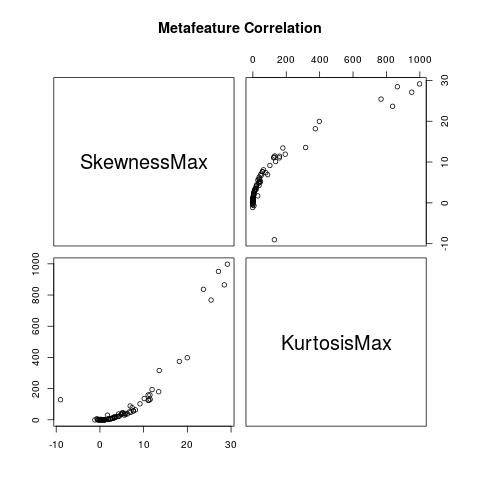
\includegraphics[width=\linewidth]{SkewnessMax_KurtosisMax_scatter.jpg}
    		\caption{Λογαριθμική συσχέτιση μεταξύ μέγιστων τιμών κυρτότητας και ασυμμετρίας} \label{fig:a}
    	\end{subfigure}\hspace*{\fill}
    	\begin{subfigure}{0.48\textwidth}
    		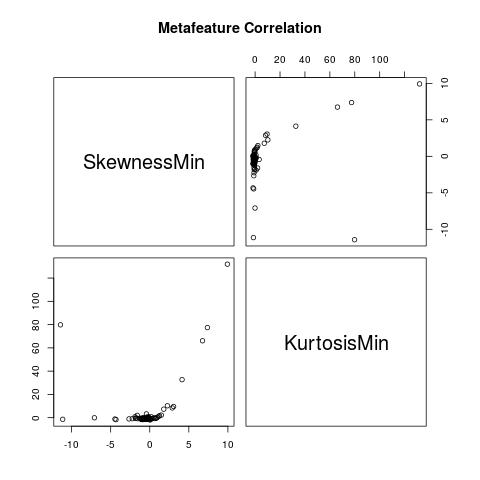
\includegraphics[width=\linewidth]{SkewnessMin_KurtosisMin_scatter.jpg}
    		\caption{Λογαριθμική συσχέτιση μεταξύ ελάχιστων τιμών κυρτότητας και ασυμμετρίας} \label{fig:b}
    	\end{subfigure}
    	
    	\medskip
    	\begin{subfigure}{0.48\textwidth}
    		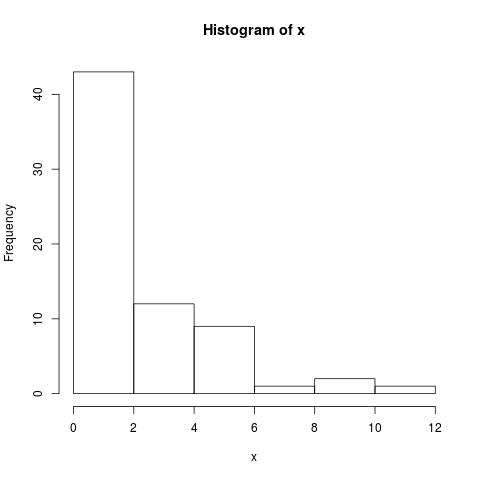
\includegraphics[width=\linewidth]{SkewnessSTD_scatter.jpg}
    		\caption{Θετική ασυμμετρία για την τυπική απόκλιση της ασυμμετρίας, όπως και για τα περισσότερα χαρακτηριστικά } \label{fig:c}
    	\end{subfigure}\hspace*{\fill}
    	\begin{subfigure}{0.48\textwidth}
    		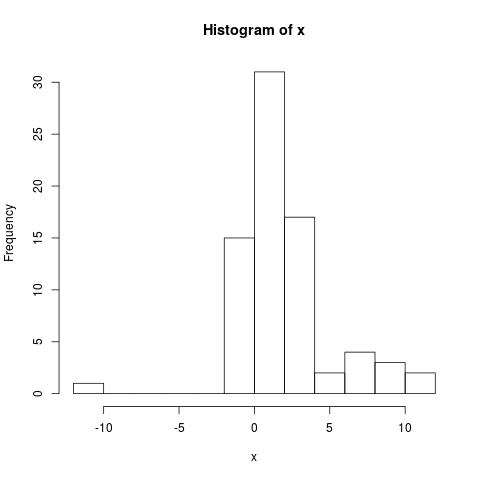
\includegraphics[width=\linewidth]{SkewnessMean_scatter.jpg}
    		\caption{Κατανομή κοντινή σε κανονική για τη μέση τιμή της ασυμμετρίας} \label{fig:d}
    	\end{subfigure}
    	
    	\medskip
    	\begin{subfigure}{0.48\textwidth}
    		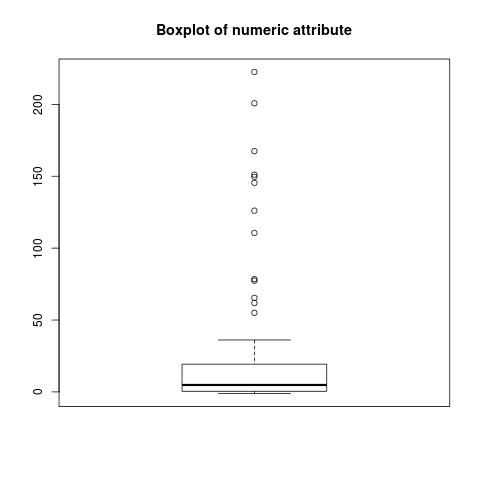
\includegraphics[width=\linewidth]{KurtosisMean_boxplot.jpg}
    		\caption{Εμφάνιση πολλών εξωκείμενων τιμών για τη μέση τιμή της κυρτότητας} \label{fig:e}
    	\end{subfigure}\hspace*{\fill}
    	\begin{subfigure}{0.48\textwidth}
    		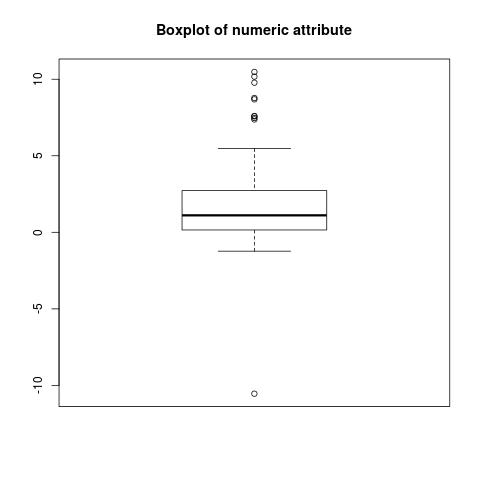
\includegraphics[width=\linewidth]{SkewnessMean_boxplot.jpg}
    		\caption{Η κανονική κατανομή της μέσης τιμής της ασσυμετρίας παρουσιάζει επίσης εξωκείμενες τιμές} \label{fig:f}
    	\end{subfigure}
    	
    	\caption{Οπτικοποίηση μετα-χαρακτηριστικών} \label{fig:1}
    \end{figure}
    
    \subsection{Επιλογή αλγορίθμου}
    Η αποθήκη σετ δεδομένων περιλαμβάνει 123 σετ δεδομένων, εκ των οποίων χρησιμοποιήθηκαν 75, καθώς τα υπόλοιπα είχαν μόνο κατηγορικά χαρακτηριστικά. Για αυτά έγινε εξαγωγή των μετα-χαρακτηρστικών και βελτιστοποίηση της υπερπαράμετρου \textit{k} του μοντέλου \textit{knn} του πακέτου \textit{caret} με χρήση του λογισμικού HPOlib \citep{hpolib} σε ένα πλέγμα αναζήτησης $K = \{\, k \mid 1 \le k \le 10 \,\}$ και τη τεχνική βελτιστοποίησης Tree Parzen   Estimator. 
    
    Αρχικά εκπαίδευτηκε ένα μοντέλο γραμμικής παλινδρόμησης με χρήση του μοντέλου \textit{lm} για αξιολόγηση της γραμμικότητας του προβλήματος. Στη συνέχεια ενσωμάτωσα στο μοντέλο μετασχηματισμό box-cox λόγω των ασυμμετριών που είχαν παρατηρηθεί κατά την ανάλυση των μεταχαρατηριστικών. Καθώς το αποτέλεσμα συνέχιζε να μην είναι ικανοποιητικό και παρατηρούνταν μοτίβα στο διάγραμμα διασποράς των residuals εξετάστηκε η χρησιμότητα ενός ισχυρότερου μοντέλου, του \textit{RadialSvm}, το οποίο υλοποιεί έναν svm με ακτινική συνάρτηση πυρήνα. 
   
   \paragraph{Χρήση ensemble με βάση τα διαστήματα πρόβλεψης.} Καθώς η απαίτηση ακριβούς πρόβλεψης της βέλτιστης τιμής μιας υπερπαραμέτρου κρίνεται, τουλάχιστον με τα τρέχοντα χαρακτηριστικά, υπερβολικά απαιτητική, όπως σχολίασαν και οι \citet{Feurer:2014:UMI:3015544.3015549}, οι οποίοι αρκέστηκαν στη χρήση των προβλέψεων τους για warmstart αλγορίθμων βελτιστοποίησης, θα χρειαστεί περαιτέρω επεξεργασία του μοντέλου. Προς αυτό το σκοπό εκμεταλλεύτηκα τα διαστήματα πρόβλεψης που παράγονται από ένα γραμμικό μοντέλο και είναι προσβάσιμα μέσω της \textit{caret}, ώστε να ορίσω ένα σύνολο βέλτιστων κ για κάθε σετ δεδομένων και να δημιουργήσω έναν ensemble με αυτά. Το σύνολο αυτό ορίζεται ως τα ακέραια κ που βρίσκονται στο $95\%$ διάστημα εμπιστοσύνης της πρόβλεψης. Αν η βέλτιστη τιμή βρίσκεται μέσα σε αυτό το διάστημα τότε με χρήση του ensemble θεωρητικά θα εξασφαλιστεί αποτέλεσμα ισάξιο με ένα μοντέλο που θα προέβλεπε επακριβώς τη βέλτιστη υπερπαράμετρο. Προϋπόθεση εγκυρότητας της παραπάνω μεθόδου είναι τα residuals να ακολουθούν κανονική κατανομή.
   
   Για τον svm η εξαγωγή των prediction intervals δεν είναι αυτοματοποιημένη. Η τεχνική που ακολουθήθηκε ήταν η εξής: υπολογισμός της διακύμανσης των residuals, εύρεση του e 95$\%$ ποσοστημορίου μιας κανονικής κατανομής με μέση τιμή $\mu$ τις προβλέψεις του μοντέλου και διακύμανση ίση με των residuals και δημιουργία του διαστήματος ως $ \interval{\mu - e}{\mu + e}$
   
   Για την εύρεση του καλύτερου αλγορίθμου χρησιμοποιήθηκαν στατιστικά τεστ. Συγκεκριμένα σύγκρινα τα σφάλματα μεταξύ των μοντέλων \textit{lm} με μετασχηματισμό box-cox, \textit{RadialSvm} και του βελτιστοποιημένου μοντέλου που παρήχθηκε από την \textit{HPOlib} στο 20$\%$ των σετ δεδομένων με χρήση του paired Wilcoxon-rank-sum τεστ σε επίπεδο εμπιστοσύνης $95\%$ για την παρατήρηση στατιστικά σημαντικών διαφορών. Ως σφάλμα ορίζω $e = 1 - accuracy$
   
   \begin{table}[!htb]
   	\begin{center}
   		\begin{tabular}{*5c}
   			\toprule
   			\multicolumn{2}{c}{Μέθοδοι} & \multicolumn{3}{c}{Υπόθεση} \\ 
   			\midrule
   			Μέθοδος 1 & Μέθοδος 2 & Δίπλευρη & Αριστερή & Δεξία\\
   			\midrule
   			svm & HPOlib & 0.0673 & 0.971 & 0.0381 \\
   			lm & HPOlib & 0.1353 & 0.9406 & 0.0673 \\
   			svm & lm & 0.09058 & 0.9608 & 0.04529 \\
   			\midrule   				
   		\end{tabular}    
   	\end{center}
   	\caption{Στατιστική σύγκριση μεθόδων}\label{mfs}
   \end{table}
   
   Με βάση τα παραπάνω στοιχεία συμπεραίνω πως:
   \begin{itemize}
   	\item Δεν μπορώ να απορρίψω την υπόθεση της μηδενικής διαφοράς μεταξύ οποιοδήποτε μεθόδων.
   	\item Μπορώ οριακά να απορρίψω τη μονόπλευρη υπόθεση ότι το μοντέλο svm έχει μεγαλύτερο σφάλμα από το βέλτιστο.
   	\item Επίσης οριακά απορρίπτω την υπόθεση ότι το μοντέλο svm έχει μεγαλύτερο σφάλμα από το μοντέλο lm.
   \end{itemize}
   
   Για τα τελικά πειράματα θα επιλέξω το μοντέλο με boxcox μετασχηματισμό, καθώς παρουσιάζει οριακά χειρότερη συμπεριφορά από το svm, αλλά είναι απλούστερο.
   
   \section{Περιγραφή τελικού μοντέλου}
   
   \subsection{Αξιολόγηση μοντέλου πρόβλεψης βελτιστοποιημέων k}
   
   Στη συνέχεια αξιολογούμε την ικανότητα του μοντέλου lm με boxcox μετασχηματισμό 
   Στα σχήματα φαίνεται ότι τα residuals του τελικού μοντέλου ακολουθούν σχετικά κανονική κατανομή, επομένως η χρήση των prediction intervals είναι έγκυρη.
   
   \begin{figure}[!htb]
   	\centering
   	\begin{minipage}{.5\textwidth}
   		\centering
   		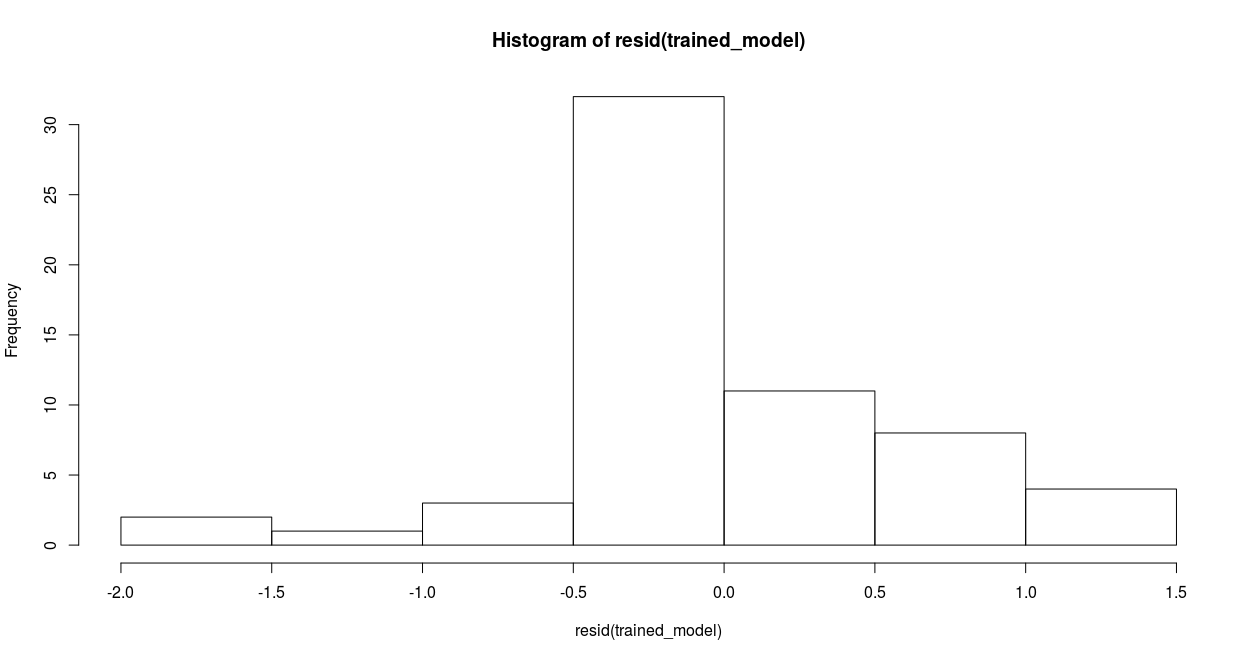
\includegraphics[width=\linewidth, height=0.2\textheight]{lm_trans_res_box}
   		\caption{Ιστόγραμμα residuals}
   		\label{fig:1}
   	\end{minipage}%
   	\begin{minipage}{0.5\textwidth}
   		\centering
   		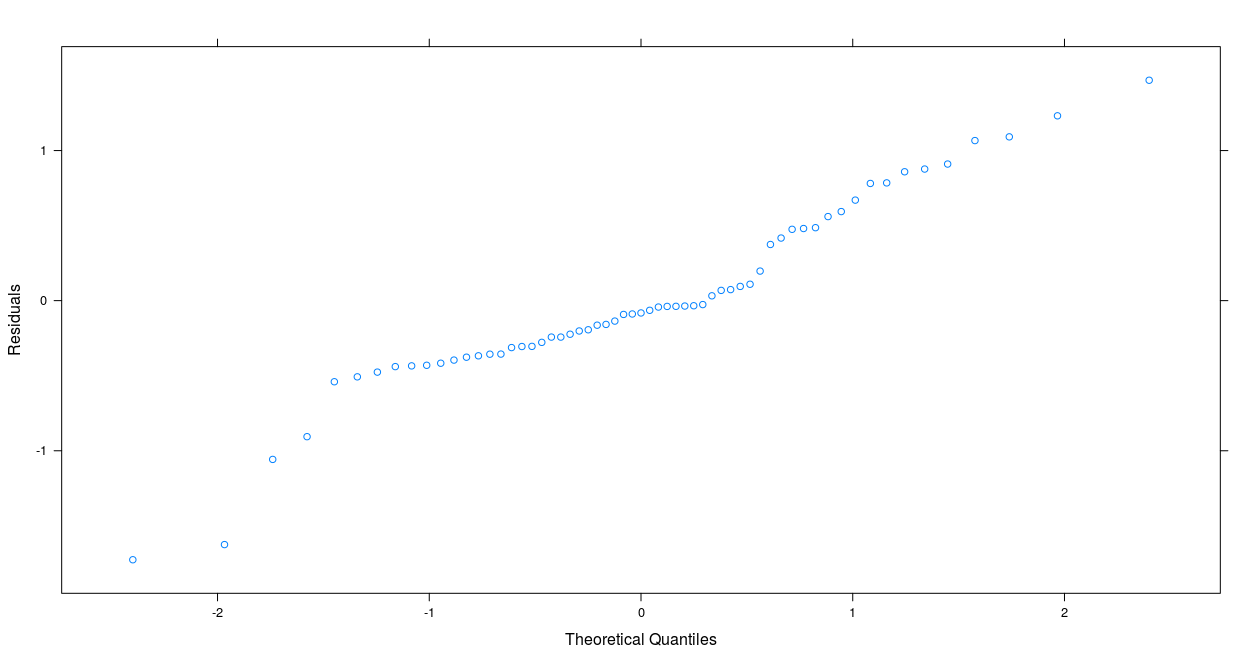
\includegraphics[width=\linewidth, height=0.2\textheight]{lm_trans_resid_qq}
   		\caption{Q-Q διάγραμμα}
   		\label{fig: 2}
   	\end{minipage}
   \end{figure}
   
   Εφαρμόζωντας την τεχνική με τα prediction intervals στο σετ ελέγχου παρατηρούμε ότι πάντα συμπεριλαμβάνουμε τη βέλτιστη λύση
   	\begin{figure}
   		\centering
   		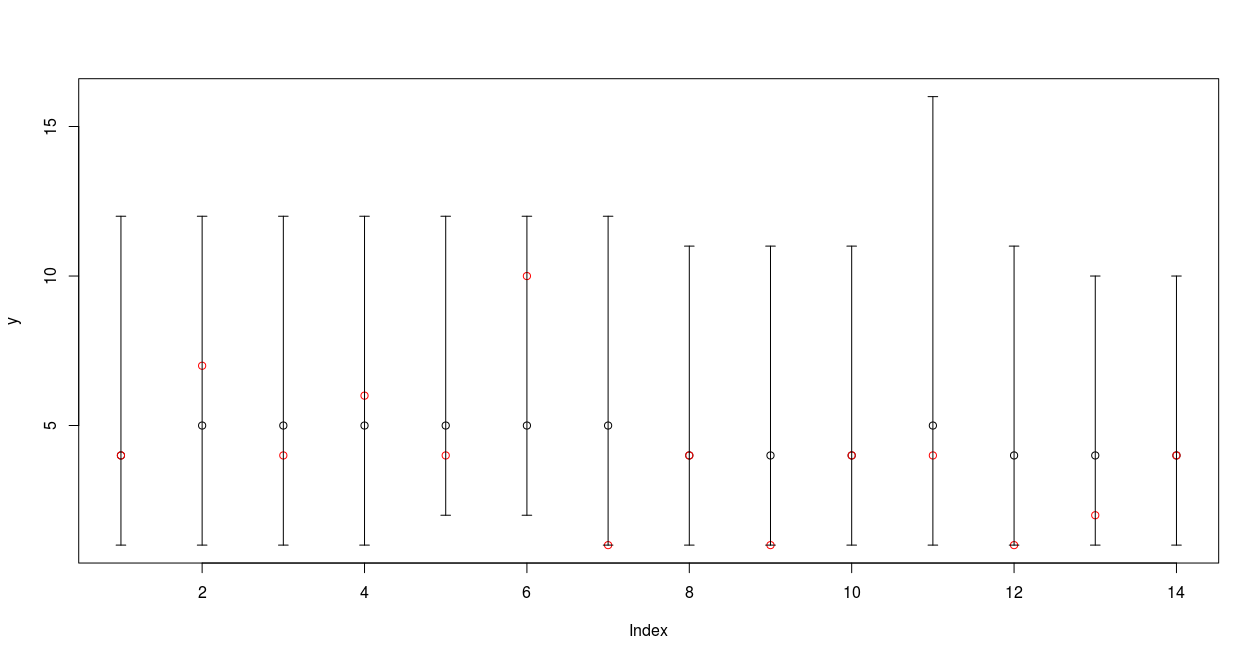
\includegraphics[width=\linewidth, height=0.15\textheight]{lm_trans_pred_int}
   		\caption{Διάγραμμα διασποράς προβλέψεων με prediction intervals }
   		\label{fig:1}
   	\end{figure}%
   	
   	\subsection{Αξιολόγηση ensemble}   	
   	H αξιολόγηση του ensemble που παράγεται με βάση το βέλτιστο μοντέλο πρόβλεψης βελτιστοποιημένων κ και τη τεχνική model selection. Εφαρμόζεται στο $20\%$ του αρχικού σετ δεδομένων, καθώς η εκπαίδευση έγινε στο υπόλοιπο $80\%$. Μετρήθηκε η ακρίβεια (accuracy) και συγκρίθηκε με αυτή που παρήχθηκε από την HPOlib (η οποία αντιστοιχεί στην ακρίβεια με βελτιστοποιημένο k).
   	
   	Η μηδενική υπόθεση δεν απορρίφθηκε με  paired Wilcoxon-rank-sum τεστ, καθώς το p-value ήταν 0.6949. 
   	
   	Ακολουθεί το διάγραμμα απόδοσης (\textit{performance plot}) \citep{Dolan2002} από το οποίο συμπεραίνουμε πως το δικό μας μοντέλο είναι πιθανότερα το βέλτιστο. 
   	
   	\begin{figure}[H]
   		\centering
   		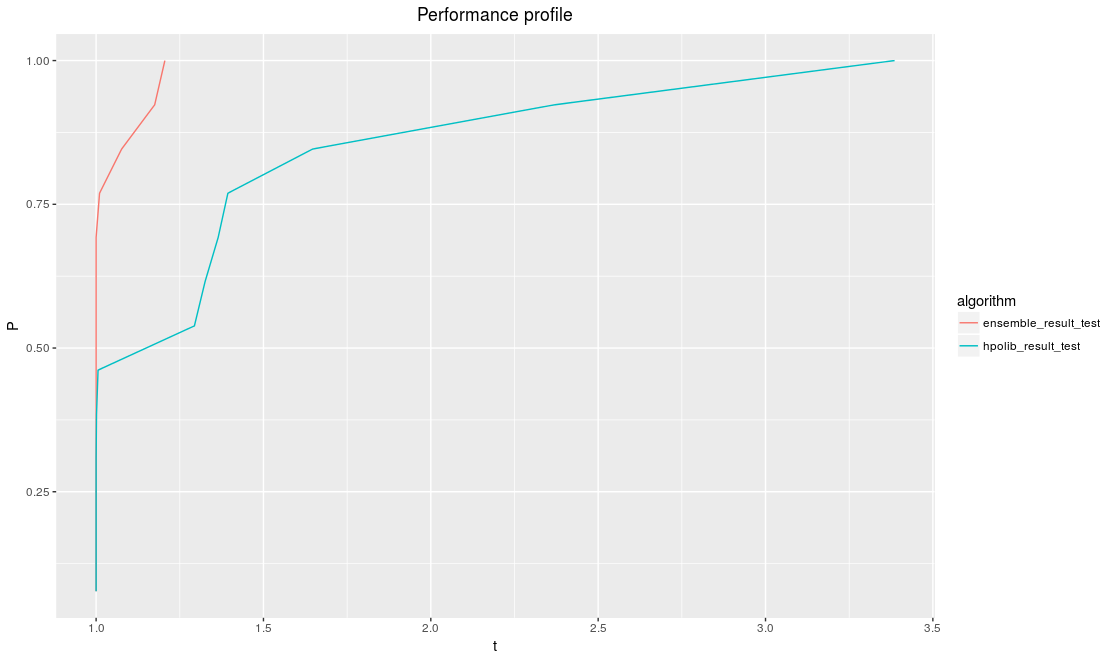
\includegraphics[width=\linewidth, height=0.3\textheight]{perf_prof}
   		\caption{Διάγραμμα απόδοσης για σύγκριση χρήσης προτεινόμενου μοντέλου με βελτιστοποιημένου HPOlib}
   		\label{fig:1}
   	\end{figure}%
   	
   	
    \printbibliography[title= Βιβλιογραφία]
\end{document}